\documentclass{standalone}
\usepackage{tikz}
%------------tikz Setup------------

\tikzstyle{ball} = [circle,shading=ball, ball color=black,
    minimum size=1mm,inner sep=1.3pt]
\tikzstyle{miniball} = [circle,shading=ball, ball color=black,
    minimum size=1mm,inner sep=0.5pt]
\tikzstyle{mminiball} = [circle,shading=ball, ball color=black,
    minimum size=0.6mm,inner sep=0.1pt]
\usetikzlibrary{arrows.meta}
\usetikzlibrary{angles, quotes}
\tikzset{>={Latex[length=2mm,width=1.5mm]}}
\tikzset{->-/.style={decoration={markings, mark=at position #1 with
  {\arrow{>}}},postaction={decorate}}}
\usetikzlibrary{decorations.pathmorphing}
\usetikzlibrary{decorations.pathreplacing}
\usetikzlibrary{arrows.meta,calc}
\usetikzlibrary{bending}
\usetikzlibrary{decorations.markings,shapes.geometric}
\tikzset{->-/.style={decoration={markings, mark=at position #1 with
  {\arrow{>}}},postaction={decorate}}}
\tikzset{-|-/.style={decoration={markings, mark=at position #1 with
  {\arrow{stealth}}},postaction={decorate}}}
\tikzset{movearrow/.style 2 args ={
        decoration={markings,
    mark= at position {#1} with {\arrow{#2}} ,
        },
        postaction={decorate}
    }
}


\begin{document}
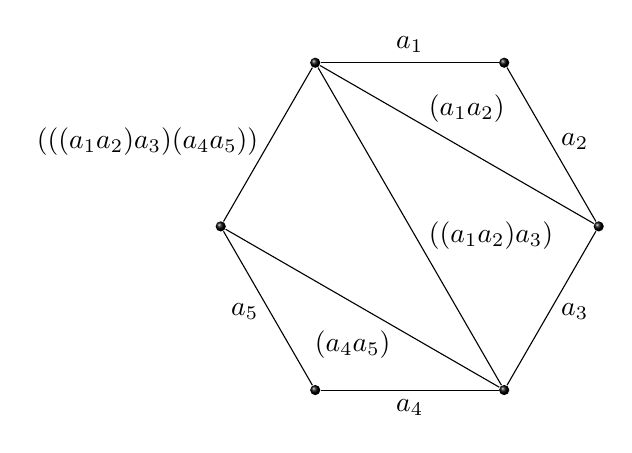
\begin{tikzpicture}
\begin{scope}[scale=1.2]
    %vertices
    \node[ball] (1) at (-1, 1.732) {};
    \node[ball] (2) at (1, 1.732) {};
    \node[ball] (3) at (2, 0) {};
    \node[ball] (4) at (1, -1.732) {};
    \node[ball] (5) at (-1, -1.732) {};
    \node[ball] (6) at (-2, 0) {};
    %edges
    \draw (1) to (2);
    \draw (2) to (3);
    \draw (3) to (4);
    \draw (4) to (5);
    \draw (5) to (6);
    \draw (6) to (1);
    %triangulations
    \draw (1) to (3);
    \draw (1) to (4);
    \draw (6) to (4);
    %labels
    \node[above] at (0,1.732) {$a_1$};
    \node[right] at (1.5,0.9) {$a_2$};
    \node[above right] at (0.1,1) {$(a_1a_2)$};
    \node[right] at (1.5,-0.9) {$a_3$};
    \node[right] at (0.1,-0.1) {$((a_1a_2)a_3)$};
    \node[below] at (0,-1.732) {$a_4$};
    \node[left] at (-1.5,-0.9) {$a_5$};
    \node[below left] at (-0.1,-1) {$(a_4a_5)$};
    \node[left] at (-1.5,0.9) {$(((a_1a_2)a_3)(a_4a_5))$};
\end{scope}
\end{tikzpicture}
\end{document}